\section{EXPERIMENTS}\label{sec:experiments}
%%%%%%%%%%%%%%%%%%%%%%%%%%%%%%%%%%%%%%%%%%%

To investigate the performance of our algorithm, we performed an extensive benchmark against the following competitors:
\begin{itemize}[noitemsep]
  \item Alternating Direction Method of Multipliers (\texttt{ADMM})~\parencite{boyd2010}.
  We considered several alternative for the choice of the augmented Lagragian parameter: an adaptive method to update the parameter throughout the algorithm~\parencite[Sec. 3.4.1]{boyd2010} and fixed values.
  In the following sections, we only kept the \texttt{ADMM} solver with a fixed value of $100$ for the augmented Lagrangian parameter.
  We present in \Cref{sec:admm-benchmarks} a more detailed benchmarks for \texttt{ADMM} solvers with different values of this parameter and the adaptive setting.
  Choosing this parameter is not straightforward and the best value changes across datasets and regularization strengh.
  \item Anderson acceleration for proximal gradient descent (\texttt{anderson PGD})~\parencite{zhang2020}
  \item Proximal Gradient Descent (\texttt{PGD})~\parencite{combettes2005}
  \item Fast Iterative Shrinkage-Thresholding Algorithm (\texttt{FISTA})~\parencite{beck2009}
  \item Semismooth Newton-Based Augmented Lagrangian (\texttt{Newt-ALM})~\parencite{Ziyan2019}

  \item The hybrid (our) solver (see \Cref{alg:hybrid}) combines proximal gradient descent
        and coordinate descent to overcome the non-separability of the SLOPE problem.
  \item The Oracle solver (\texttt{oracle CD}) uses the clusters obtained via another solver to compute coordinate descent updates from the known solver.
  Note that it cannot be used in practice as it requires identifying the clusters of the minimizer of the SLOPE optimization problem \Cref{pb:slope}. This solver solves \Cref{pb:separable_slope} where clusters are obtained with the \texttt{hybrid} solver.
\end{itemize}

We used \pkg{Benchopt}~\parencite{moreau2022benchopt} to obtain the convergence curves for the different solvers.
\pkg{Benchopt} is a collaborative framework that allows reproducible and automatic benchmarks.
% This would void anonymity. We should uncomment for the camera-ready version.
% The repository to reproduce the benchmark is available at \url{https://github.com/Klopfe/benchmark_slope}.
The repository to reproduce the benchmark is available in the supplementary material.

Unless we note otherwise, we used the Benjamini--Hochberg method to compute the \(\lambda\) sequence~\parencite{bogdan2015},
which sets $\lambda_j = \eta^{-1}(1 - q\times j / (2p))$ for $j=1, 2, \hdots, p$ where $\eta^{-1}$ is the probit function.
For the rest of the experiments section, the parameter $q$ of this sequence has been set to $0.1$ if not stated otherwise.\footnote{We initially experimented with various settings for \(q\) but found that they made little difference to the relative performance of the algorithms.}
We let \(\lambda_\text{max}\) be the \(\lambda\) sequence such that \(\beta^* = 0\), but for which any scaling with a strictly positive scalar smaller than one produces a solution with at least one non-zero coefficient.
We then parameterize the experiments by scaling \(\lambda_\text{max}\), using the fixed factors \(1/2\), \(1/10\), and \(1/50\), which together cover the range of very sparse solutions to the almost-saturated case.

We pre-process datasets by first removing features with less than three non-zero values. Then, for dense data we center and scale each feature by its mean and standard deviation respectively.
For sparse data, we scale each feature by its maximum absolute value.

Each solver was coded in \pkg{python}, using \pkg{numpy}~\parencite{harris2020} and \pkg{numba}~\parencite{lam2015} for performance-critical code.
The code will be made open-source upon publication and is available in the supplementary material.
In \Cref{sec:solver-details}, we provide additional details on the implementations of some of the solvers used in our benchmarks.

The computations were carried out on a computing cluster with dual Intel Xeon CPUs (28 cores) and 128 GB of RAM.

\subsection{Simulated Data}
\label{sec:experiments-real-data}

\begin{figure*}[!t]
  \centering
  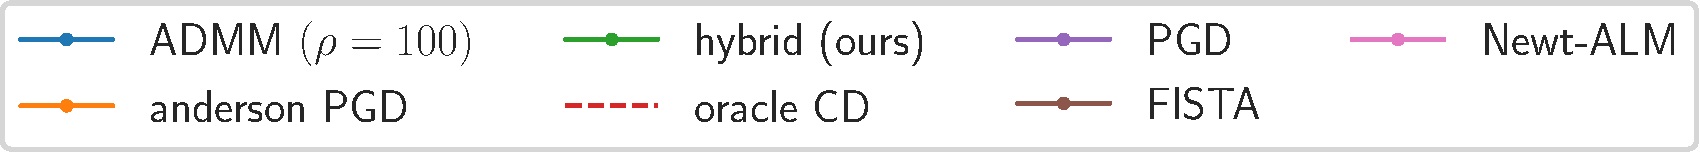
\includegraphics{simulated_legend.pdf}
  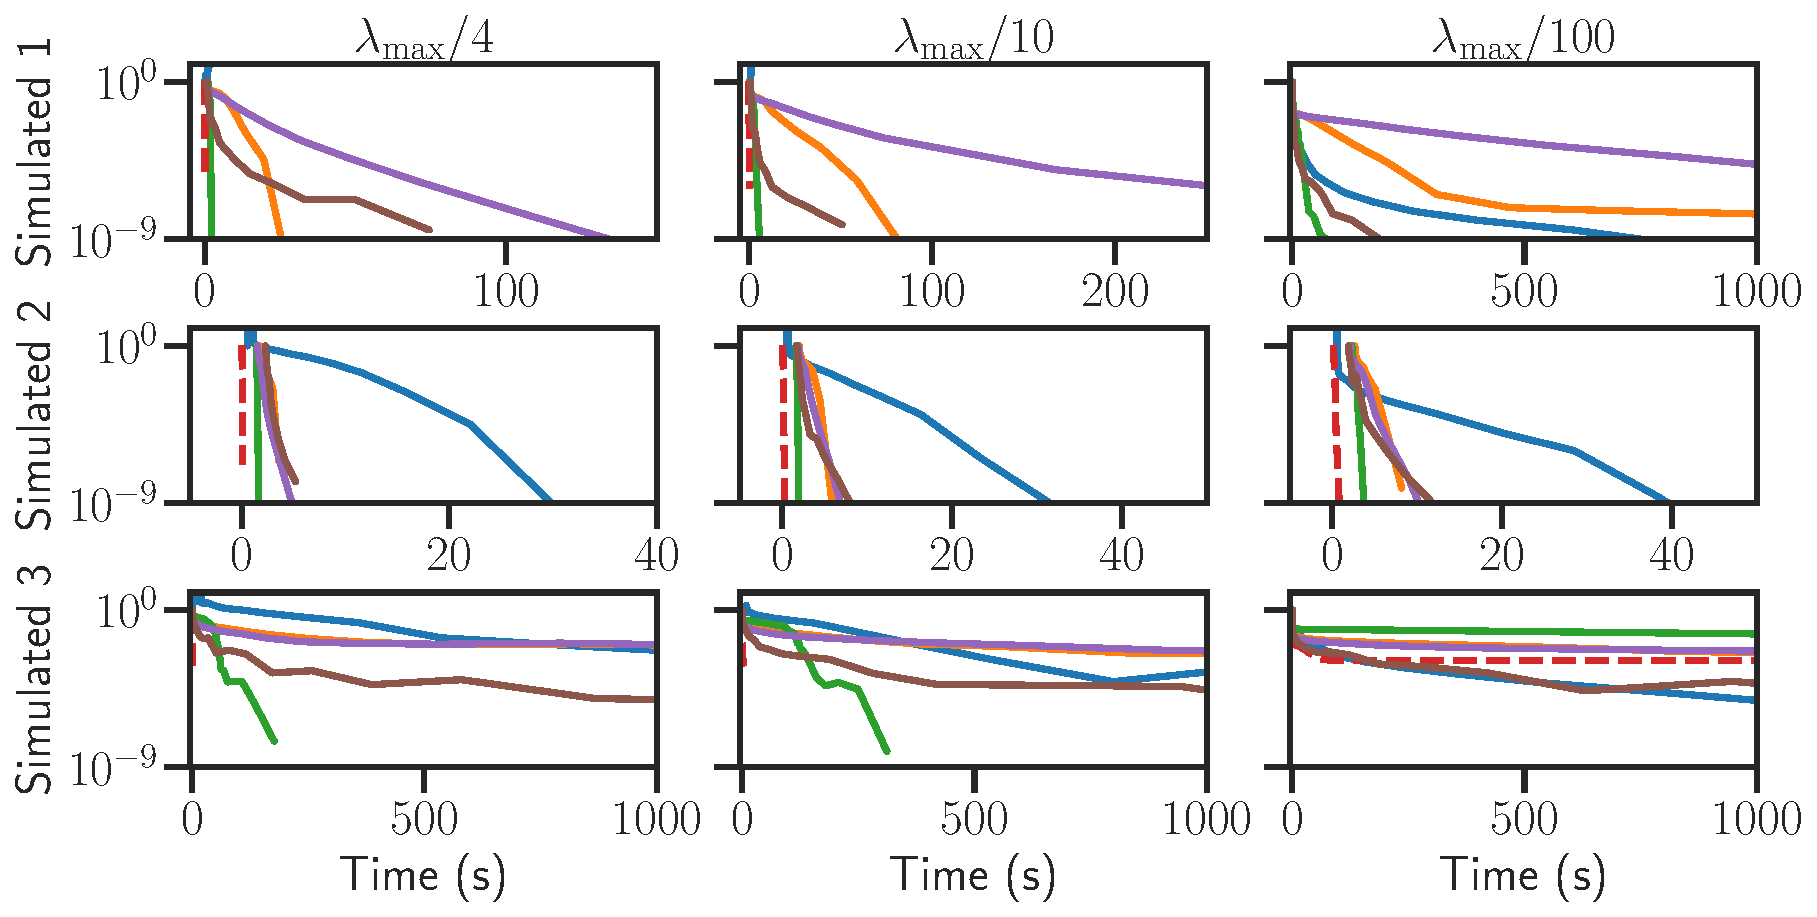
\includegraphics[scale=0.9]{simulated.pdf}
  \caption{Benchmark on simulated datasets. The plots show suboptimality as a function of time for SLOPE on multiple simulated datasets and $\lambda$ sequences of varying strength.}
  \label{fig:simulated}
\end{figure*}

The design matrix $X$ was generated such that features had mean one and unit variance, with correlation between features $j$ and $j'$ equal to $0.6^{|j-j'|}$.
%where $\rho$ is a parameter that can be chosen in $[0, 1[$.
%We fixed this value at $0.6$.
We generated \(\beta \in \mathbb{R}^p\) such that \(k\) entries, chosen uniformly at random throughout the vector, were sampled from a standard Gaussian distribution.
The response vector, meanwhile, was set to $y=X\beta + \varepsilon$, where
$\varepsilon$ was sampled from a multivariate Gaussian distribution with variance such that $\lVert X\beta\rVert / \lVert \varepsilon \rVert = 3$.
The different scenarios for the simulated data are described in \Cref{tab:simulated-data}.

\begin{table}[hbt]
  \centering
  \caption{Scenarios for the simulated data in our benchmarks}
  \label{tab:simulated-data}
  \begin{tabular}{
      l
      S[table-format=5.0,round-mode=off]
      S[table-format=7.0,round-mode=off]
      S[table-format=2.0,round-mode=off]
      S[table-format=1.3,round-mode=off]
    }
    \toprule
    {Scenario} & {\(n\)} & {\(p\)} & {\(k\)} & {Density} \\ \midrule
    1          & 200     & 20000   & 20      & 1         \\
    2          & 20000   & 200     & 40      & 1         \\
    3          & 200     & 200000 & 20      & 0.001     \\ \bottomrule
  \end{tabular}
\end{table}

In \Cref{fig:simulated}, we present the results of the benchmarks on simulated data.
We see that for smaller fractions of $\lambda_{\text{max}}$ our hybrid algorithm allows significant speedup in comparison to its competitors mainly when the number of features is larger than the number of samples.
On very large scale data such as in simulated data setting $3$, we see that the hybrid solver is faster than its competitors by one or two orders of magnitude.


For the second scenario, notice that all solvers take considerably longer than the \texttt{oracle CD} method to reach convergence.
This gap is a consequence of Cholesky factorization in the case of \texttt{ADMM} and computation of \(\norm{X}_2\) in the remaining cases.
For the hybrid method, we can avoid this cost, with little impact on performance, since \(\norm{X}_2\) is used only in the PGD step.

\subsection{Real data}
\label{sec:experiments-real-data}



The datasets used for the experiments have been described in \Cref{tab:real-data} and were obtained from \textcite{chang2011,chang2016,breheny2022}.

\begin{table}[hbt]
  \centering
  \caption{%
    List of real data sets used in our experiments.
    See \Cref{tab:dataset-sources} in \Cref{sec:dataset-sources} for references on these datasets.
  }
  \label{tab:real-data}
  \begin{tabular}{
      l
      S[table-format=5.0,round-mode=off]
      S[table-format=7.0,round-mode=off]
      S[table-format=1.5,round-mode=figures,round-precision=2]
    }
    \toprule
    Dataset            & {\(n\)} & {\(p\)} & {Density} \\ \midrule
    \dataset{bcTCGA}   & 536     & 17322   & 1         \\
    \dataset{news20}   & 19996   & 1355191 & 0.0003357 \\
    \dataset{rcv1}     & 20242   & 44504   & 0.00166   \\
    \dataset{Rhee2006} & 842     & 360     & 0.02469   \\ \bottomrule
  \end{tabular}
\end{table}

\Cref{fig:real-data} shows the suboptimality for the objective function $P$ as a function of the time for the four different datasets.
We see that when the regularization parameter is set at $\lambda_{\text{max}}/2$ and $\lambda_{\text{max}}/10$, our proposed solver is faster than all its competitors---especially when the datasets become larger.
This is especially visible for the \dataset{news20} dataset where we see that our proposed method is faster by at least one order of magnitude.

\begin{figure*}[!t]
  \centering
  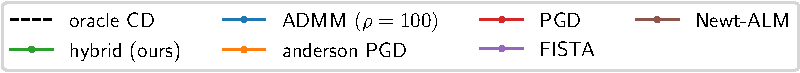
\includegraphics{real_legend.pdf}
  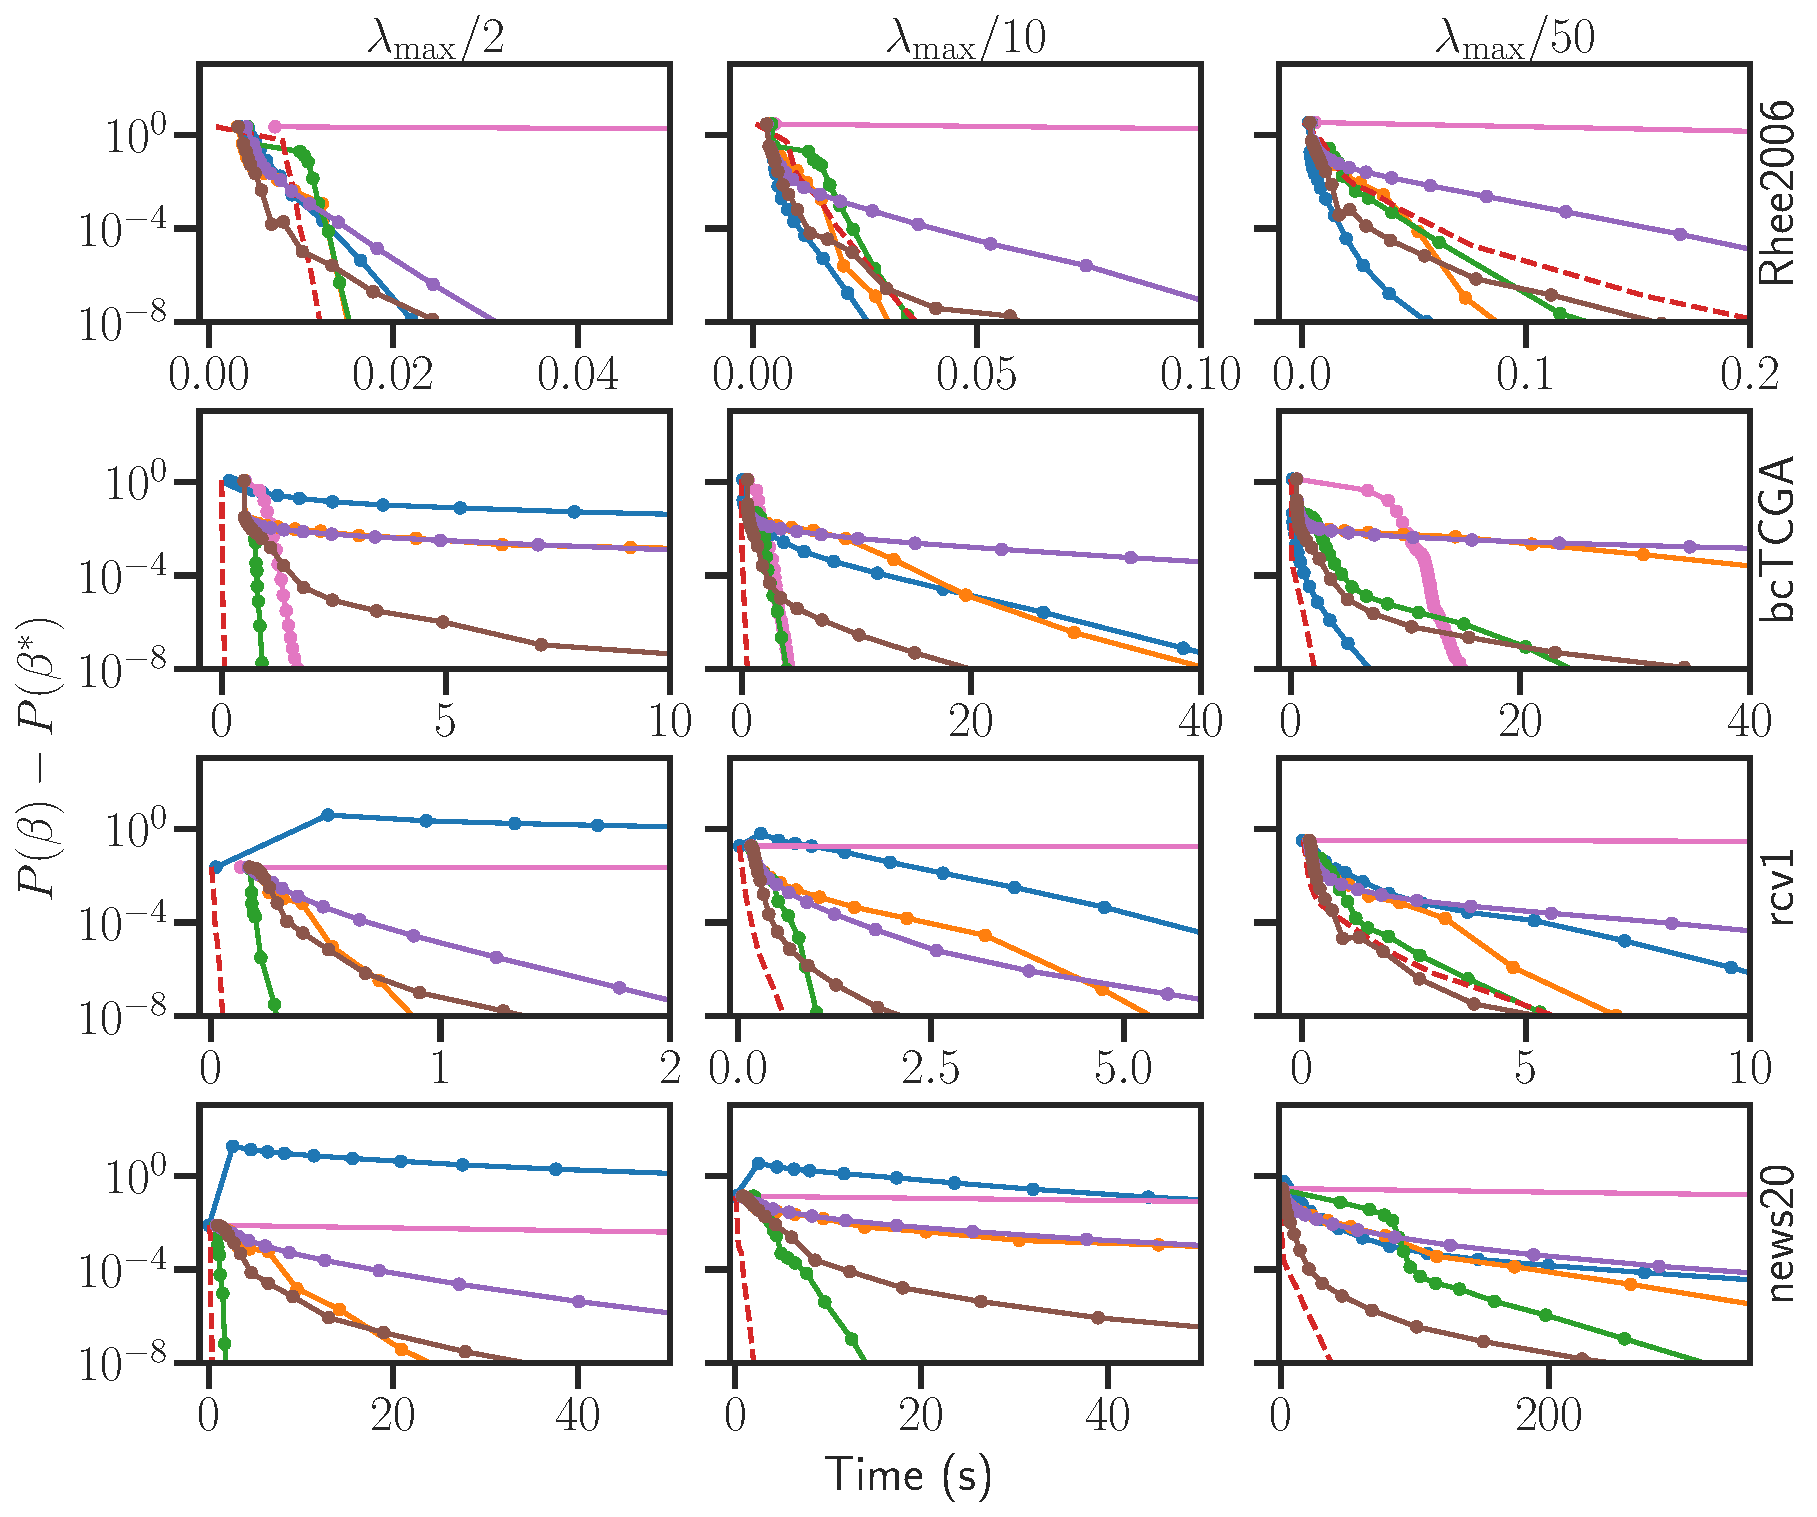
\includegraphics[scale=0.9]{real.pdf}
  \caption{Benchmark on real datasets. The plots show suboptimality as a function of time for SLOPE on multiple simulated datasets and $\lambda$ sequences of varying strength.}
  \label{fig:real-data}
\end{figure*}



When the parametrization value is set to $\lambda_{\text{max}}/50$, our algorithm remains competitive on the different datasets.
It can be seen that the different competitors do not behave consistently across the datasets.
For example, the \texttt{Newt-ALM} method is very fast on the \dataset{bcTCGA} dataset but is very slow on the \dataset{news20} dataset whereas the \texttt{hybrid} method remains very efficient in both settings.
